
\section{SIAR}
\label{sec:orgea06a9c}
\index{Data!SIAR}
\index{Data!Meteorological variables}

The Agroclimatic Information System for Irrigation (SIAR)
\cite{SIAR2011} is a free-download database operating since 1999,
covering the majority of the irrigated area of Spain.  This network
belongs to the Ministry of Agriculture, Food and Environment of Spain,
as a tool to predict and study meteorological variables for
agriculture. SIAR is composed of twelve regional centers and a
national center, aiming to centralize and depurate measurements from
the stations of the network. Figure \ref{fig:SIAR_map} displays the
stations over an altitude map. Some stations from the complete network
have been omitted, due to difficulties accessing their coordinates
or to incomplete or spurious data series\footnote{The name and location data of these stations are available at the \href{https://github.com/oscarperpinan/CMSAF-SIAR/blob/master/data/SIAR.csv}{GitHub repository} of the paper \cite{Antonanzas-Torres.Canizares.ea2013}.}.
\begin{figure}
  \centering
  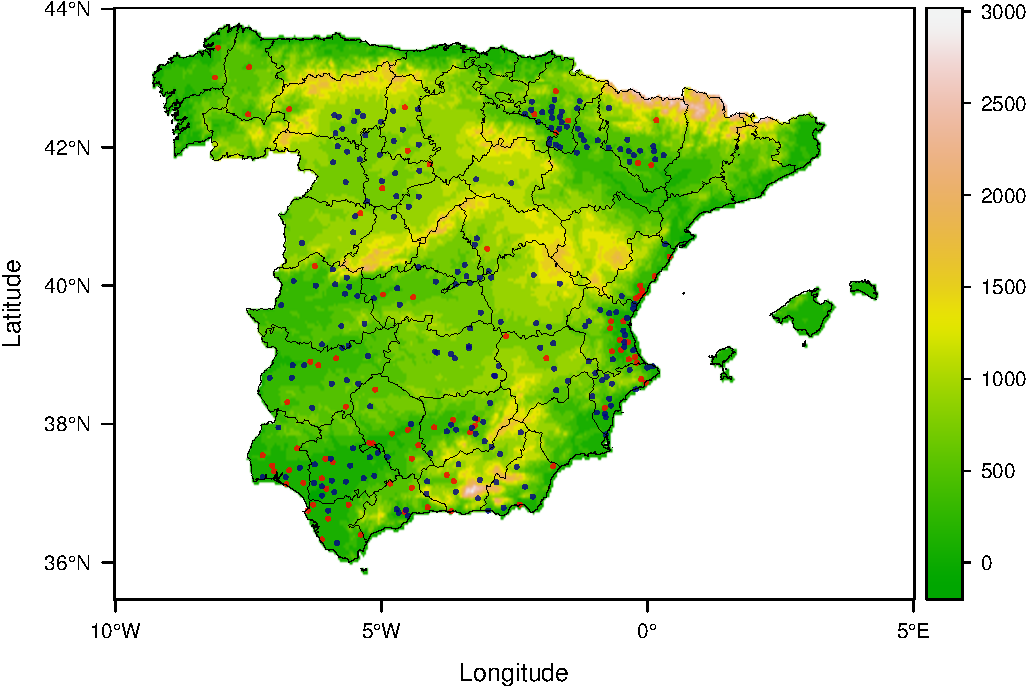
\includegraphics[width=\textwidth]{figs/mapaSIAR_crop}
  \caption{Meteorological stations of the SIAR network. The color key
    indicates the altitude (meters).}
  \label{fig:SIAR_map}
\end{figure}

\subsection{Daily Data of Different Meteorological Variables}
\label{sec:org55a588e}
As an example of multiple time series with different scales, we
will use 8 years (from January 2004 to December 2011) of daily
data corresponding to several meteorological variables measured at
the SIAR station located at Aranjuez (Madrid, Spain) available on
the SIAR webpage\footnote{\url{http://eportal.magrama.gob.es/websiar}}. The \texttt{aranjuez.gz} file, available in the
\texttt{data} folder of the book repository, contains this information
with several meteorological variables: average, maximum, and
minimum ambient temperature; average and maximum humidity; average
and maximum wind speed; rainfall; solar radiation on the
horizontal plane; and evotranspiration.

The \texttt{read.zoo} from the \texttt{zoo} package accepts this string and
downloads the data to construct a \texttt{zoo} object. Several
arguments are passed directly to \texttt{read.table} (\texttt{header}, \texttt{skip},
etc.) and are detailed conveniently on the help page of this
function. The \texttt{index.column} is the number of the column with the
time index, and \texttt{format} defines the date format of this index.

\index{Packages!zoo@\texttt{zoo}}
\index{read.zoo@\texttt{read.zoo}}

\lstset{language=r,label= ,caption= ,captionpos=b,numbers=none}
\begin{lstlisting}
  library(zoo)
  
  aranjuez <- read.zoo("data/aranjuez.gz",
                       index.column = 3, format = "%d/%m/%Y",
                       fileEncoding = 'UTF-16LE',
                       header = TRUE, fill = TRUE,
                       sep = ';', dec = ",", as.is = TRUE)
  aranjuez <- aranjuez[, -c(1:4)]
  
  names(aranjuez) <- c('TempAvg', 'TempMax', 'TempMin',
                       'HumidAvg', 'HumidMax',
                       'WindAvg', 'WindMax',
                       'Radiation', 'Rain', 'ET')
  
  
  summary(aranjuez)
\end{lstlisting}

\index{zoo@\texttt{zoo}}

From the summary it is clear that parts of these time series include erroneous outliers that can be
safely removed:
\lstset{language=r,label= ,caption= ,captionpos=b,numbers=none}
\begin{lstlisting}
  aranjuezClean <- within(as.data.frame(aranjuez),{
    TempMin[TempMin>40] <- NA
    HumidMax[HumidMax>100] <- NA
    WindAvg[WindAvg>10] <- NA
    WindMax[WindMax>10] <- NA
  })
  
  aranjuez <- zoo(aranjuezClean, index(aranjuez))
\end{lstlisting}


\subsection{Solar Radiation Measurements from Different Locations}
\label{sec:orgcf9b0ce}
As an example of multiple time series with the same scale, we will use
data of daily solar radiation measurements from different locations.

\index{Data!Solar radiation}
\index{Data!SIAR}

Daily solar radiation incident on the horizontal plane is registered
by meterological stations and estimated from satellite images. This
meteorological variable is important for a wide variety of scientific
disciplines and engineering applications. Its variations and trends,
dependent on the location (mainly latitude, and also longitude and
altitude) and on time (day of the year), have been analyzed and
modeled in a huge collection of papers and reports. In this section
we will focus our attention on the time evolution of the solar
radiation. The spatial distribution and the spatio-time behavior will
be the subject of later sections.

The stations of the SIAR network include first-class pyranometers
according to the World Meteorological Organization (WMO), whose
absolute accuracy is within \(\pm 5\%\) and is typically lower than \(\pm
3\%\). Solar irradiance is recorded every 15 minutes and then
collated through a datalogger within the station to generate the daily
irradiation, which is later sent to the regional and national centers.

The file \texttt{navarra.RData} contains daily solar radiation data of 2011
from the meteorological stations of Navarra, Spain. The names of the
dataset are the abbreviations of each station name.


\section{Unemployment in the United States}
\label{sec:org7a12f51}
As an example of time series that can be displayed both in individual
and in aggregate, we will use the unemployment data in the United
States. The information on unemployed persons by industry and class of
worker is available in Table A-14 published by the Bureau of Labor
Statistics\footnote{\url{http://www.bls.gov/webapps/legacy/cpsatab14.htm}}.

The dataset arranges the information with a row for each category
(\texttt{Series.ID}) and a column for each monthly value. In addition, there
are columns with the annual summaries (\texttt{annualCols}). We rearrange
this \texttt{data.frame}, dropping the \texttt{Series.ID} and the annual columns,
and transpose the data.

\index{Data!Unemployment}

\lstset{language=r,label= ,caption= ,captionpos=b,numbers=none}
\begin{lstlisting}
  unemployUSA <- read.csv('data/unemployUSA.csv')
  nms <- unemployUSA$Series.ID
  ##columns of annual summaries
  annualCols <- 14 + 13*(0:12)
  ## Transpose. Remove annual summaries
  unemployUSA <- as.data.frame(t(unemployUSA[,-c(1, annualCols)]))
  ## First 7 characters can be suppressed
  names(unemployUSA) <- substring(nms, 7)
  head(unemployUSA)
\end{lstlisting}

With the transpose, the column names of the original data set are
now the row names of the \texttt{data.frame}. The \texttt{as.yearmon} function
of the \texttt{zoo} package converts the character vector of names into a
\texttt{yearmon} vector, a class for representing monthly data. With
\texttt{Sys.setlocale("LC\_TIME", 'C')} we ensure that month abbreviations
(\texttt{\%b}) are correctly interpreted in a non-English locale. This
vector is the time index of a new \texttt{zoo} object. 

\index{Packages!zoo@\texttt{zoo}}
\index{as.yearmon@\texttt{as.yearmon}}
\index{apply@\texttt{apply}}
\index{zoo@\texttt{zoo}}

\lstset{language=r,label= ,caption= ,captionpos=b,numbers=none}
\begin{lstlisting}
  library(zoo)
  
  Sys.setlocale("LC_TIME", 'C')
  idx <- as.yearmon(row.names(unemployUSA), format='%b.%Y')
  unemployUSA <- zoo(unemployUSA, idx)
\end{lstlisting}

Finally, those rows with \texttt{NA} values are removed.
\lstset{language=r,label= ,caption= ,captionpos=b,numbers=none}
\begin{lstlisting}
  isNA <- apply(is.na(unemployUSA), 1, any)
  unemployUSA <- unemployUSA[!isNA,]
\end{lstlisting}

\section{Gross National Income and CO\(_{\text{2}}\) Emissions}
\label{sec:org0e2c416}
The catalog data of the World Bank Open Data initiative includes the
World Development Indicators (WDI)\footnote{\url{http://databank.worldbank.org/data/reports.aspx?source=world-development-indicators}}. Among them we will analyze
the evolution of the relationship between Gross National Income (GNI)
and \(CO_2\) emissions for a set of countries. The package \texttt{WDI} is able
to search and download these data series.

\index{Data!World Bank} 
\index{Data!CO2@$CO_2$}
\index{Data!GNI}
\index{Packages!WDI@\texttt{WDI}}

\lstset{language=r,label= ,caption= ,captionpos=b,numbers=none}
\begin{lstlisting}
  library(WDI)
    
  CO2data <- WDI(indicator=c('EN.ATM.CO2E.PC', 'EN.ATM.CO2E.PP.GD',
                'NY.GNP.MKTP.PP.CD', 'NY.GNP.PCAP.PP.CD'),
            start=2000, end=2011,
            country=c('BR', 'CN', 'DE', 'ES',
                'FI', 'FR', 'GR', 'IN', 'NO', 'US'))

  names(CO2data) <- c('iso2c', 'Country.Name', 'Year',
                      'CO2.capita', 'CO2.PPP',
                      'GNI.PPP', 'GNI.capita')
\end{lstlisting}

Only two minor modifications are needed: Remove the missing values and
convert the \texttt{Country.Name} column into a \texttt{factor}. This first
modification will save problems when displaying the time series, and
the \texttt{factor} conversion will be useful for grouping.
\lstset{language=r,label= ,caption= ,captionpos=b,numbers=none}
\begin{lstlisting}
  isNA <- apply(is.na(CO2data), 1, any)
  CO2data <- CO2data[!isNA, ]

  CO2data$Country.Name <- factor(CO2data$Country.Name)
\end{lstlisting}
